\subsection{Iterazioni}
Il team seguirà la metodologia di progetto RUP, in seguito sono specificati il piano di progetto e le
iterazioni che lo compongono.

\subsection{Piano}
Il piano di progetto si suddivide in 4 fasi temporali:
\begin{itemize}
    \item Inizio
    \item Elaborazione
    \item Costruzione
    \item Transizione
\end{itemize}
Le attività coinvolte sono le seguenti:
\begin{itemize}
    \item Studio di fattibilità
    \item Raccolta dei requisiti
    \item Analisi e progetto
    \item Implementazione
    \item Test
\end{itemize}
Le varie attività si andranno a distribuire sulle fasi temporali, con una distribuzione eterogenea, che
dipende da quanto una particolare attività è significativa in una certa fase.\\
Qui sotto è raffigurato il processo in un grafico descrittivo:

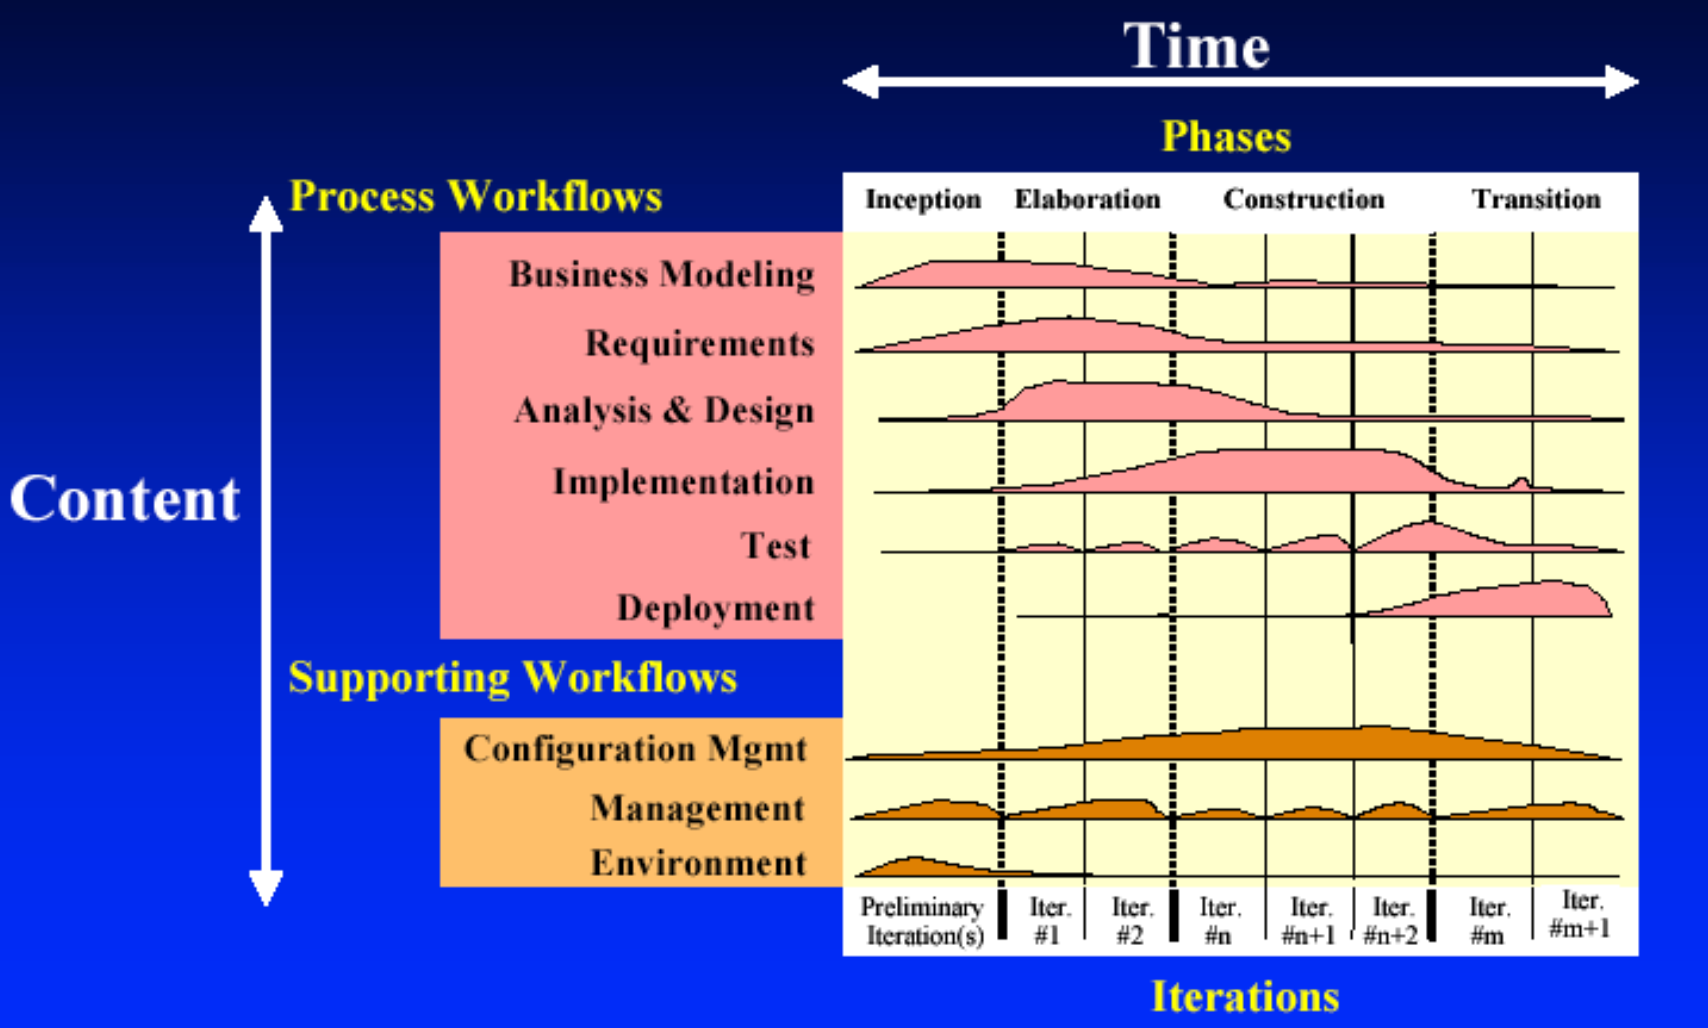
\includegraphics[width=12cm]{images/RUPplan.png}

\subsection{Iterazioni}